%% bare_jrnl.tex
%% V1.3
%% 2007/01/11
%% by Michael Shell
%% see http://www.michaelshell.org/
%% for current contact information.
%%
%% This is a skeleton file demonstrating the use of IEEEtran.cls
%% (requires IEEEtran.cls version 1.7 or later) with an IEEE journal paper.
%%
%% Support sites:
%% http://www.michaelshell.org/tex/ieeetran/
%% http://www.ctan.org/tex-archive/macros/latex/contrib/IEEEtran/
%% and
%% http://www.ieee.org/

%%*************************************************************************
%% Legal Notice:
%% This code is offered as-is without any warranty either expressed or
%% implied; without even the implied warranty of MERCHANTABILITY or
%% FITNESS FOR A PARTICULAR PURPOSE! 
%% User assumes all risk.
%% In no event shall IEEE or any contributor to this code be liable for
%% any damages or losses, including, but not limited to, incidental,
%% consequential, or any other damages, resulting from the use or misuse
%% of any information contained here.
%%
%% All comments are the opinions of their respective authors and are not
%% necessarily endorsed by the IEEE.
%%
%% This work is distributed under the LaTeX Project Public License (LPPL)
%% ( http://www.latex-project.org/ ) version 1.3, and may be freely used,
%% distributed and modified. A copy of the LPPL, version 1.3, is included
%% in the base LaTeX documentation of all distributions of LaTeX released
%% 2003/12/01 or later.
%% Retain all contribution notices and credits.
%% ** Modified files should be clearly indicated as such, including  **
%% ** renaming them and changing author support contact information. **
%%
%% File list of work: IEEEtran.cls, IEEEtran_HOWTO.pdf, bare_adv.tex,
%%                    bare_conf.tex, bare_jrnl.tex, bare_jrnl_compsoc.tex
%%*************************************************************************

\documentclass[journal]{IEEEtran}


\usepackage{amsmath,
            amssymb,
            amsthm,
            atbegshi,
            caption,
            subcaption,
            epigraph,
            etoolbox,
            enumitem,
            fancyhdr,
            geometry,
            graphicx,
            hyperref,
            kpfonts,
            lipsum,
            longtable,
            natbib,
            tabulary,
            thmtools,
            tikz,
            tikzpagenodes,
            titletoc,
            titlesec,
            tocloft,
            url,
            wrapfig
}
\usepackage[utf8]{inputenc}

% correct bad hyphenation here
\hyphenation{op-tical net-works semi-conduc-tor}

\begin{document}
%
% paper title
% can use linebreaks \\ within to get better formatting as desired
\title{Report A*}

\author{Anders Sildnes, Andrej Leitner~\IEEEmembership{students }% <-this % stops a space. jobtitle in memberkj
}% \thanks{Utsendt 2014}}

% The paper headers
\markboth{A* stuff}%
{h}

% make the title area
\maketitle

\begin{abstract}
    This text answers assignment 1
    this is some more text that I can probably fill in somehow.
    Hello my name is alfred.
\end{abstract}

% \begin{IEEEkeywords}
%     Stuff
% \end{IEEEkeywords}
\IEEEPARstart{A*}{} is a local search algorithm. It is similar to DFS and BFS,
except that when choosing a new node, it always chooses a node based on an 
index value. 

\section{Method}
Since A* always chooses either the lowest or highest cost for a node, we desided
to implement the queue with a heap. All heaps have the property that the root
node has a consistenly higher or a lower value than all of its children. In addition,
insertions are $\log{n}$, so maintaining such a queue is relatively fast. A 
regular list would cost at least $n \log{n}$ for sorting.

A* star is a method that should work equally on all \textit{problems}. A problem needs
to maintain a list of \textit{states}. Since problem and states is the only 
variying input, we decided to model these using different classed and objects.

While python does not have the strict notion of abstract classes, we created
a superclass ``Problem'' and an abstract superclass ``State''. These have
general methods to be used in A*. The methods are listed in \autoref{fig:UMLproblem}.
Explanation:

In the \textit{Problem} class, the network 
\begin{description}
    \item[network] is a reference to the (currently) cartesian
    plane of vertices and edges. 
    \item[Destructor] is invoked after the queue of states is exhausted (clean-up and animation).
        We included this since some animations will e.g.\ paint the goal node as
        a part of a path rather than a final state, etc.
    \item[genNeighbour()] will genereate all possible successor states
        from the current state
    \item[triggerstart] generates a starting state to be used in A*
    \item[updateStates] paints and animates the next state. In the next state
        is a direct successor, we often dont need to paint every other state.
\end{description}

\begin{figure}[Hb]
\centering
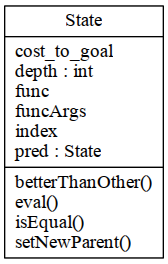
\includegraphics[height=5cm,keepaspectratio,width=2.5in]{fig/problem.png}%
\caption{UML Class diagram for a problem instance}
\label{fig:UMLproblem}
\end{figure}

In \autoref{fig:UMLstate}, you will find the following:
\begin{description}
    \item[func,funcargs:] when propagating and updating old states, I found it
        useful if all states had some knowledge of their own function and arguments.
        This is redundant (since often the function is the same in all states),
        but easier to read.
    \item[betterThanOther] is the function equivalent of the \textless operator,
        used to compare states.
\end{description}

What can be seen from the abstract classes and framework is that none of the code
mentions the exact type of problem to be solved. This means the code can be used
to model any problem that has an iteratively progressing scheme.

\section{A*}
The assignment description models an A* search as follows:
\begin{enumerate}
    \item pop the currently most promising state.
    \item generate all possbile successor states
    \item if a successor state has a similar index value or position:
        \begin{enumerate}
            \item if the successor state is better:
                \begin{enumerate}
                    \item set the remembered state to this index such that future
                        discoveries point to this successor
                \end{enumerate}
            \item 
        \end{enumerate}
\end{enumerate}

All states need a method to be indexed. This index should be similar between
states at the same point. This means that the heuristic function returns the same
value. The objective function, however, usually measured as the depth, can be
different. In general we want the shortest path, so whenever two states
have the same index, the one with the shortes ancestor tree is remembered
as the state for the index, and the other is forgotten.
In our case, the index value (assumed to be an integer) is stored in a dictionary.
The lookup, and insertions are $O(1)$.

Since each successor will need to have an objective value, we use the objective
function \textit{attach-and-eval} whenever generating a successor. Similar to 
the A*-code given in the assignment text, we do not actually evaluate the 
state until it is popped off the queue.

\section{Generating successor states}
In a classical problem like search, we cannot generate completely random
states. This would essentially be forking the problem in two: instead of only
looking for the goal, we are now also looking for a path to the start.
Other situations, does not necessarily require that you find an optimal path,
e.g.\ the 8-queens puzzle. Here, you could make random choices and easilier
find a valid solution.

Since the generation of successor states seems to depend on the problem, we
opted with saying that the implementation of \textit{genSuccessors} should be done
for each problem. We could say that an A* search should just reason 
with its states and ``state-children'', but we felt this would clutter
more than help.

To keep it general, the generation of successor states is kept



\section{Comparison of heuristic functions}
In this assignment, we were supposed to find the shortest path
from a point $S$ to a point $D$ on 2D-grid. This topic is widely discussed in other
literature, so I will not elaborate.

A common heuristic function is the \textit{manhattan distance}, which measures the 
distance from a point $P: (x_{i},y_{i})$ to $D: (x_{j},y_{j})$, by taking the difference
between $x_i, x_j$ summed with the difference between $y_i, y_j$. Here, $x_j,y_j$ is 
the goal we are trying to reach, and $x_i, y_i$  is the current point of the A*
search.
The downside of the manhattan distance is that it does not circumfere obstacles.
Consider figure \autoref{fig:manhattansucks}

\begin{figure}[Hb]
\centering
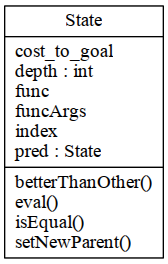
\includegraphics[height=5cm,keepaspectratio,width=2.5in]{fig/problem.png}%
\caption{Case where the manhattan algorithm does not fare well.}
\label{fig:manhattansucks}
\end{figure}

Other common heuristics, also used




\begin{figure}[Hb]
\centering
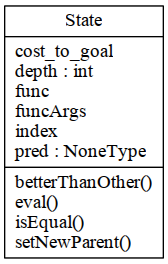
\includegraphics[height=5cm,keepaspectratio,width=2.5in]{fig/state.png}%
\caption{UML Class diagram for a state instance}
\label{fig:UMLstate}
\end{figure}


% An example of a double column floating figure using two subfigures.
%\begin{figure*}[!t]
%\centerline{\subfloat[Case I]\includegraphics[width=2.5in]{subfigcase1}%
%\label{fig_first_case}}
%\hfil
%\subfloat[Case II]{\includegraphics[width=2.5in]{subfigcase2}%
%\label{fig_second_case}}}
%\caption{Simulation results}
%\label{fig_sim}
%\end{figure*}
%

% An example of a floating table. Note that, for IEEE style tables, the 
% \caption command should come BEFORE the table. Table text will default to
% \footnotesize as IEEE normally uses this smaller font for tables.
% The \label must come after \caption as always.
%
\begin{table}[!t]
% increase table row spacing, adjust to taste
\renewcommand{\arraystretch}{1.3}
% if using array.sty, it might be a good idea to tweak the value of
% \extrarowheight as needed to properly center the text within the cells
\caption{Comparison of nodes generated}
\label{table_example}
\centering
% Some packages, such as MDW tools, offer better commands for making tables
% than the plain LaTeX2e tabular which is used here.
\begin{tabular}{|c|ccc|}
\hline
DFS & 1 & 100 & 110 \\
\hline
BFS & 9123 & 123 & daw \\
\hline
BeFS & 9123 & 123 &* dwa \\
\hline
\end{tabular}
\end{table}

\begin{table}[!t]
% increase table row spacing, adjust to taste
\renewcommand{\arraystretch}{1.3}
% if using array.sty, it might be a good idea to tweak the value of
% \extrarowheight as needed to properly center the text within the cells
\caption{Lengths of solution paths}
\label{table_example}
\centering
% Some packages, such as MDW tools, offer better commands for making tables
% than the plain LaTeX2e tabular which is used here.
\begin{tabular}{|c|ccc|}
\hline
DFS & 1 & 100 & 110 \\
\hline
BFS & 9123 & 123 & daw \\
\hline
BeFS & 9123 & 123 &* dwa \\
\hline
\end{tabular}
\end{table}


\begin{IEEEbiographynophoto}{Anders Sildnes,}
    4.års student, master informatikk, NTNU.\
\end{IEEEbiographynophoto}
\begin{IEEEbiographynophoto}{Andrej Leitner,}
    4.års student, master informatikk, NTNU.\
\end{IEEEbiographynophoto}

    
% if have a single appendix: %\appendix[Proof of the Zonklar Equations]
% or
%\appendix  % for no appendix heading
% do not use \section anymore after \appendix, only \section*
% is possibly needed
% \appendices
% \section{Proof of the First Zonklar Equation}
% Appendix one text goes here.
%\bibliographystyle{IEEEtran}
%\bibliography{IEEEabrv,../bib/paper}
%
% \begin{thebibliography}{1}
%
% \bibitem{IEEEhowto:kopka}
% H.~Kopka and P.~W. Daly, \emph{A Guide to \LaTeX}, 3rd~ed.\hskip 1em plus
%   0.5em minus 0.4em\relax Harlow, England: Addison-Wesley, 1999.
%
% \end{thebibliography}
% biography section
% 
% If you have an EPS/PDF photo (graphicx package needed) extra braces are
% needed around the contents of the optional argument to biography to prevent
% the LaTeX parser from getting confused when it sees the complicated
% \includegraphics command within an optional argument. (You could create
% your own custom macro containing the \includegraphics command to make things
% simpler here.)
%\begin{biography}[{\includegraphics[width=1in,height=1.25in,clip,keepaspectratio]{mshell}}]{Michael Shell}
% or if you just want to reserve a space for a photo:
\end{document}
